The main text of the report starts here. The format is rather free. It should be absolutely fine to write something here before the first section.

\section{The First Section}

% This is not a topic sentence, started vague.
Starting with a topic sentence. The first section is probably an introduction section where the background of this research project is introduced. It would be nice to have a little equation:

\begin{equation}
    (A,Z) \rightarrow (A,Z+2) + 2e^- + 2\Bar{\nu}_e + Q_{\beta\beta},
\end{equation}

\noindent no indent here because the equation is not the end of a paragraph but it is not always true. Here what everything mean in the equation should be explained. A figure just like Figure \ref{fig:bb} might be helpful for explaining the equation. And a little citation \cite{Moe:2014ioa} because why not. Now we can have a second equation: 

\begin{equation}\label{eq:0nubd}
    (A,Z) \rightarrow (A,Z+2) + 2e^- + Q_{\beta\beta}.
\end{equation}

This time a new paragraph is started and there is no need to put \textbackslash noindent at the begining.

\begin{figure}[h]
\begin{center}
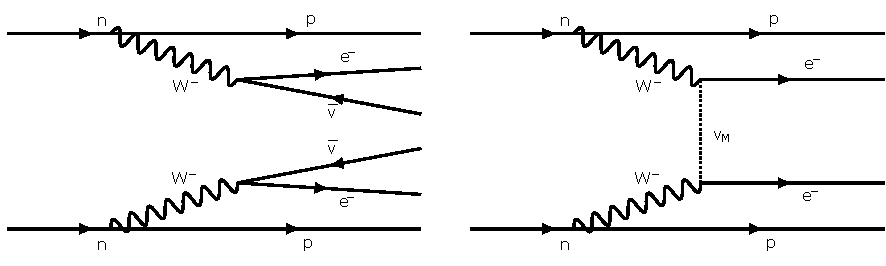
\includegraphics[width=15cm]{figures/2vbb_0vbb.pdf}
\end{center}
\caption{Caption.}\label{fig:bb}
\end{figure}


\subsection{Subsection}

Content here.

\subsection{Another subsection}

Content here. And a table (Table \ref{tbl:curLimit}). 

\begin{table}
\caption{\label{tbl:curLimit} $T_{1/2}^{0\nu}$ and $\langle m_{\beta\beta} \rangle$ limits (90\% C.L.) from selected recent 
measurements, sorted by the mass number. The $\langle m_{\beta\beta} \rangle$ limits are listed as reported in 
refereed publications. Adapted form \cite{Dolinski:2019nrj} }
\begin{center} 
\begin{tabular}{llll} \\ \hline\hline
Isotope           &  T$_{1/2}^{0\nu}$ ($\times 10^{25}$~y)                       & $\langle m_{\beta\beta}\rangle$ (eV)     &  Experiment\\ \hline
$^{76}$Ge         &  $>8.0$                       &  $<0.12-0.26$                          &  GERDA~\cite{Agostini:2018tnm} \\
                      &   $>1.9$                       &  $<0.24-0.52$                     &  {\sc Majorana Demonstrator}~\cite{Aalseth:2017btx}  \\
$^{130}$Te         &  $>1.5$                       &  $<0.11-0.52$                       &  CUORE~\cite{Alduino:2017ehq}\\
$^{136}$Xe      &  $>10.7$                       &  $<0.061-0.165$                       &  KamLAND-Zen~\cite{KamLAND-Zen:2016pfg} \\ 
    &  $>1.8$                       &  $<0.15-0.40 $                       &  EXO-200~\cite{Albert:2017owj} \\  \hline
\end{tabular}
\end{center}
\end{table}

\section{The Second Section}

Content here.

\subsection{Subsection}

Content here.

\subsection{Subsection 2}

Content here.

\section{The Third Section}

Content here.

\subsection{Subsection}

Content here.

\subsection{One more subsection}

Content here.

\section{Future Works}

Write about research projects that is going to be in a PhD thesis here.

\subsection{One project}

The first project for PhD thesis.

\subsection{Another project}

Something else. Change the bibliography style if you do not like it.